% !TeX root = ../main.tex

% Edit this title for each week's entry.
\section{Week 5 - Comparison Methods}

\topic{Project Relationships and Alternatives}

\begin{definition}[Investment (``Project'')]
    An exchange of resources now for expected benefits in the future.
\end{definition}
\b{Objective}: evaluate and compare projects when there are multiple
solutions or opportunities. It is important to consider how these projects
are \b{related} to each other: \rb{independent}, \rb{mutually exclusive},
or \rb{related but not mutually exclusive}.

\begin{definition}[Independent]
    The expected costs and benefits of each project \b{do not depend} on
    whether or not the other one is chosen.
\end{definition}

\begin{example}[Home Improvement Projects]
    Paint a room, build a fence, replace the toilet, buy patio furniture,
    \dots
    \\\db{Each one is a separate yes/no decision.}
\end{example}

\begin{definition}[Mutually Exclusive]
    When one project is chosen, \b{all the other ones are excluded}.
\end{definition}

\begin{example}[Buying a Car]
    You only need one car: buy a Honda Civic, a Toyota Camry, a Volkswagen
    Jetta, or a Lexus RX, \dots
    \\\db{Picking one excludes the rest.}
\end{example}

\begin{definition}[Related but Not Mutually Exclusive]
    \begin{itemize}
        \item \b{Not mutually exclusive}: you can select more than one
        \item \b{Related}: selecting one may affect the selection of another option
    \end{itemize}
    A common cause is a budget limitation.
\end{definition}

\begin{example}[Reflection: Budget Limits]
    \begin{center}
    \begin{tabular}{lr}
        \toprule
        Project & Budget \\
        \midrule
        1. Paint room & \$5000 \\
        2. Build a fence & \$7000 \\
        3. Replace toilet & \$6000 \\
        4. Buy patio furniture & \$3000 \\
        \bottomrule
    \end{tabular}
    \end{center}
    How would you describe the relationship between these projects if your
    total budget is\dots
    \begin{enumerate}[label = \alph*)]
        \item \$1,000,000?
        \\\db{Independent: all four together cost only \$21,000, so the budget never binds.}
        \item \$7,000?
        \\\db{Mutually exclusive: the two cheapest together cost $\$5000 + \$3000 = \$8000 > \$7000$, so you can afford at most one.}
        \item \$10,000?
        \\\db{Related but not mutually exclusive: some pairs fit (e.g.\ 1 \& 4), but choosing one project limits which others you can add.}
    \end{enumerate}
\end{example}

\heading{How to Decide on Projects}
\begin{itemize}
    \item \b{Independent} $\to$ consider each option separately
    \item \b{Mutually exclusive} $\to$ find the best option
    \item \b{Related but not mutually exclusive} $\to$ form \rb{mutually exclusive alternatives} (combinations), then find the best one
\end{itemize}

\begin{example}[Mutually Exclusive Combinations]
    Same four projects with a limited budget of \$10,000. What are the
    mutually exclusive combinations?
    \\\db{List every combination that fits within the budget (including doing nothing):}
    \begin{center}
    \begin{tabular}{clr}
        \toprule
        Alternative & Projects & Cost \\
        \midrule
        0 & Do nothing & \$0 \\
        1 & 1 & \$5000 \\
        2 & 2 & \$7000 \\
        3 & 3 & \$6000 \\
        4 & 4 & \$3000 \\
        5 & 1 + 4 & \$8000 \\
        6 & 2 + 4 & \$10{,}000 \\
        7 & 3 + 4 & \$9000 \\
        \bottomrule
    \end{tabular}
    \end{center}
    \db{1 + 2 (\$12,000), 1 + 3 (\$11,000), 2 + 3 (\$13,000) and anything larger exceed the budget. Exactly one of these 8 alternatives is chosen, so they are mutually exclusive.}
\end{example}

\heading{Summary}
\begin{enumerate}
    \item Multiple projects can be \b{independent}, \b{mutually exclusive}, or \b{related but not mutually exclusive}
    \item Related projects are handled by forming mutually exclusive combinations
\end{enumerate}

\topic{Present Worth and Annual Worth}

\heading{Project Cash-flows}
\begin{center}
    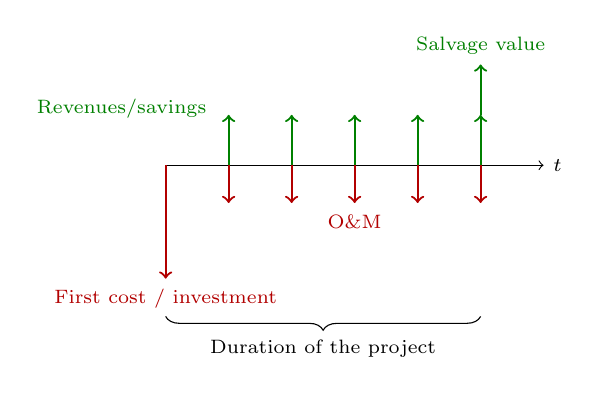
\begin{tikzpicture}[scale=0.8]
        \draw[->] (0,0) -- (6,0) node[right] {\scriptsize $t$};
        \draw[->,thick,red!70!black] (0,0) -- (0,-1.8) node[below] {\scriptsize First cost / investment};
        \foreach \x in {1,...,5}{
            \draw[->,thick,green!50!black] (\x,0) -- (\x,0.8);
            \draw[->,thick,red!70!black] (\x,0) -- (\x,-0.6);
        }
        \draw[->,thick,green!50!black] (5,0.8) -- (5,1.6) node[above] {\scriptsize Salvage value};
        \node[green!50!black,left] at (0.8,0.9) {\scriptsize Revenues/savings};
        \node[red!70!black] at (3,-0.9) {\scriptsize O\&M};
        \draw[decorate,decoration={brace,mirror,amplitude=5pt}] (0,-2.4) -- (5,-2.4) node[midway,below=5pt] {\scriptsize Duration of the project};
    \end{tikzpicture}
\end{center}
\db{These are discounted using some rate. Which one?}

\begin{definition}[MARR]
    The \rb{Minimum Acceptable Rate of Return}: based on risk and/or the
    expected rate of return from the \b{best alternative}. Also known as
    the \rb{hurdle rate}: projects that earn less than MARR are not
    acceptable.
\end{definition}

\begin{remark}
    Assume money can \textbf{always} be invested at MARR. This means that
    \textbf{doing nothing} is earning at MARR.
\end{remark}

\begin{definition}[Present Worth (PW)]
    Also called \rb{Net Present Value (NPV)}: the present value of
    benefits $-$ costs, discounted at MARR. For \b{independent} projects:
    \begin{itemize}
        \item $\text{PW} > 0 \to$ acceptable
        \item $\text{PW} < 0 \to$ unacceptable
    \end{itemize}
\end{definition}

\begin{remark}
    The PW of a project is ``the amount by which this project is beating
    the best alternative, expressed in today's value.''
\end{remark}

\begin{example}[Calculating PW]
    You plan to buy a Honda Civic with a life of 10 years; MARR is 5\%. The
    annual benefits are worth \$4000 and the annual costs \$1000. The first
    cost is \$20,000 and the salvage value after 10 years is \$4000. What is
    the PW?
    \\\db{Net annual benefit $= 4000 - 1000 = \$3000$:}
    \begin{align*}
        \text{PW} &= -20{,}000 + 3000(P/A,5\%,10) + 4000(P/F,5\%,10)\\
        &= -20{,}000 + 3000(7.7217) + 4000(0.61391) = \db{\$5621}
    \end{align*}
    \db{$\text{PW} > 0$, so buying the car is acceptable.}
\end{example}

\begin{definition}[Annual Worth (AW)]
    The \b{equivalent annuity} of PW:
    \[\boxed{\text{AW} = \text{PW}(A/P,\text{MARR},N)}\]
    For \b{independent} projects:
    \begin{itemize}
        \item $\text{AW} > 0 \to$ acceptable
        \item $\text{AW} < 0 \to$ unacceptable
    \end{itemize}
\end{definition}

\begin{example}[Annual Worth of Car]
    Honda Civic: FC \$20,000, annual benefits $-$ costs \$3000, life 10
    years, salvage \$4000, MARR 5\%.
    \\\db{Convert each cash-flow to an annuity directly:}
    \begin{align*}
        \text{AW} &= -20{,}000(A/P,5\%,10) + 3000 + 4000(A/F,5\%,10)\\
        &= -20{,}000(0.12950) + 3000 + 4000(0.07950) = \db{\$728}
    \end{align*}
    \db{Check: $5621(A/P,5\%,10) = 5621(0.12950) = \$728$.}
\end{example}

\heading{Summary}
\begin{enumerate}
    \item MARR is the rate of return of the best alternative, used as the ``hurdle'' rate
    \item PW is the present value of all costs/benefits discounted at MARR; AW is its equivalent annuity
    \item Independent projects: accept if $\text{PW} > 0$ (equivalently $\text{AW} > 0$)
\end{enumerate}

\topic{Evaluating Mutually Exclusive Projects (PW/AW)}

\heading{Mutually Exclusive Projects}
We can only choose one option, so we must choose the \b{best}. Steps to
evaluate projects with PW:
\begin{enumerate}
    \item Define the \b{time horizon}
    \item Develop the cash-flows for each alternative
    \item Calculate the PW using MARR
    \item Compare the PWs and pick the best
\end{enumerate}

\begin{remark}
    ``Do nothing'' is always an alternative when no better choice is
    available (i.e.\ if all options have $\text{PW} < 0$).
\end{remark}

\begin{example}[Mutually Exclusive Projects with Same Lives]
    \begin{center}
    \begin{tabular}{lrr}
        \toprule
        & Honda Civic & Tesla Model S \\
        \midrule
        FC & \$20,000 & \$100,000 \\
        Annual benefits $-$ cost & \$3000 & \$12,000 \\
        Life & 10 years & 10 years \\
        Salvage value & \$4000 & \$14,000 \\
        MARR & 5\% & 5\% \\
        \bottomrule
    \end{tabular}
    \end{center}
    \db{Both lives are 10 years, so compare PWs directly:}
    \begin{align*}
        \text{PW}_H &= -20{,}000 + 3000(P/A,5\%,10) + 4000(P/F,5\%,10) = \$5621\\
        \text{PW}_T &= -100{,}000 + 12{,}000(7.7217) + 14{,}000(0.61391) = \$1256
    \end{align*}
    \db{Both beat doing nothing, but $\text{PW}_H > \text{PW}_T$: \dbb{buy the Honda Civic}.}
\end{example}

\heading{PW Comparison for Different Lives}
What if the lives (and so the time horizons) differ? Consider buying a
toothbrush: one costs \$5 and lasts 2 years, the other costs \$4 and lasts
1 year.
\\\db{Comparing \$5 against \$4 directly is unfair: the \$4 one only covers half the time. We need a common time horizon.}

\begin{definition}[Repeated Lives]
    Assume each project \b{repeats itself} (e.g.\ you always need a
    car/toothbrush). Compare over the \rb{least common multiple (LCM)} of
    the individual lives.
\end{definition}

\begin{center}
    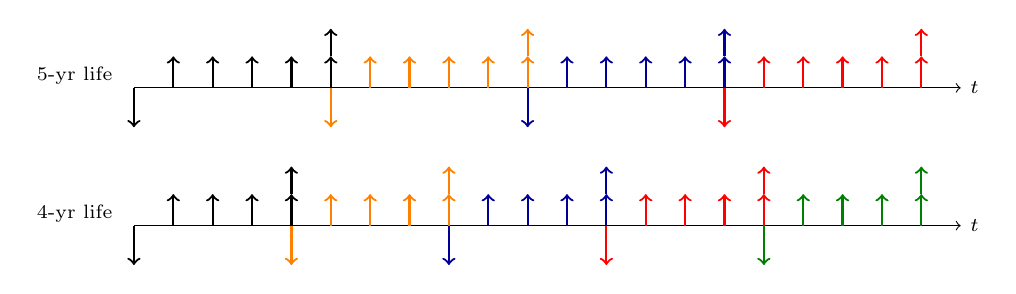
\begin{tikzpicture}[scale=0.5]
        % 5-year project repeated 4x over 20 years
        \draw[->] (0,0) -- (21,0) node[right] {\scriptsize $t$};
        \draw[->,thick] (0,0) -- (0,-1);
        \foreach \c/\s in {black/0,orange/5,blue!60!black/10,red/15}{
            \foreach \k in {1,...,5}{\draw[->,thick,\c] (\s+\k,0) -- (\s+\k,0.8);}
            \draw[->,thick,\c] (\s+5,0.8) -- (\s+5,1.5);
        }
        \foreach \x/\c in {5/orange,10/blue!60!black,15/red}{\draw[->,thick,\c] (\x,0) -- (\x,-1);}
        \node[left] at (-0.3,0.3) {\scriptsize 5-yr life};
        % 4-year project repeated 5x over 20 years
        \begin{scope}[yshift=-3.5cm]
        \draw[->] (0,0) -- (21,0) node[right] {\scriptsize $t$};
        \draw[->,thick] (0,0) -- (0,-1);
        \foreach \c/\s in {black/0,orange/4,blue!60!black/8,red/12,green!50!black/16}{
            \foreach \k in {1,...,4}{\draw[->,thick,\c] (\s+\k,0) -- (\s+\k,0.8);}
            \draw[->,thick,\c] (\s+4,0.8) -- (\s+4,1.5);
        }
        \foreach \x/\c in {4/orange,8/blue!60!black,12/red,16/green!50!black}{\draw[->,thick,\c] (\x,0) -- (\x,-1);}
        \node[left] at (-0.3,0.3) {\scriptsize 4-yr life};
        \end{scope}
    \end{tikzpicture}
    \\[2pt] \textit{\small Lives of 5 and 4 years both repeat to fill the LCM of 20 years}
\end{center}

\begin{example}[PW (Repeated Lives)]
    \begin{center}
    \begin{tabular}{lrr}
        \toprule
        & Honda Civic & Lexus RX \\
        \midrule
        FC & \$20,000 & \$40,000 \\
        Annual benefits $-$ cost & \$3000 & \$8000 \\
        Life & 10 years & \b{5 years} \\
        Salvage value & \$4000 & \$13,000 \\
        MARR & 5\% & 5\% \\
        \bottomrule
    \end{tabular}
    \end{center}
    \db{LCM of 10 and 5 is 10 years, so the Lexus is bought twice. At $t = 5$ it is sold for \$13,000 and replaced for \$40,000, a net $-\$27{,}000$:}
    \begin{align*}
        \text{PW}_L &= -40{,}000 + 8000(P/A,5\%,10) + 13{,}000(P/F,5\%,10) - 27{,}000(P/F,5\%,5)\\
        &= -40{,}000 + 8000(7.7217) + 13{,}000(0.61391) - 27{,}000(0.78353)\\
        &= \$8600
    \end{align*}
    \db{$\text{PW}_H = \$5621$ (from before). $\text{PW}_L > \text{PW}_H$: \dbb{buy the Lexus RX}.}
\end{example}

\heading{AW of Repeated Lives}
We can also compare options using AW (the equivalent annuity of PW). A
repeated project has the \b{same} AW in every cycle, so the AW over one life
equals the AW over the LCM.

\begin{remark}
    Comparing AW is equivalent to comparing PW of repeated projects, and
    only needs \textbf{one life} of each project.
\end{remark}

\begin{example}[AW (Repeated Lives)]
    Same Honda Civic and Lexus RX.
    \begin{align*}
        \text{AW}_H &= -20{,}000(A/P,5\%,10) + 3000 + 4000(A/F,5\%,10) = \$728\\
        \text{AW}_L &= -40{,}000(A/P,5\%,5) + 8000 + 13{,}000(A/F,5\%,5)\\
        &= -40{,}000(0.23097) + 8000 + 13{,}000(0.18097) = \$1114
    \end{align*}
    \db{$\text{AW}_L > \text{AW}_H$: \dbb{buy the Lexus RX}, the same decision as PW. Check: $8600(A/P,5\%,10) = \$1114$.}
\end{example}

\begin{definition}[Study Period]
    Adopt a \b{specified time period} for comparison (e.g.\ when projects
    will not be repeated), and \b{adjust the salvage value} of any project
    whose life extends past the study period.
\end{definition}

\begin{center}
    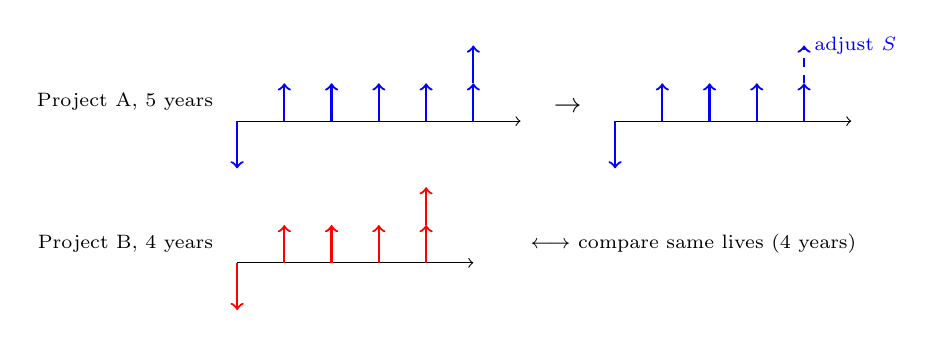
\begin{tikzpicture}[scale=0.6]
        \node[left] at (-0.3,0.4) {\scriptsize Project A, 5 years};
        \draw[->] (0,0) -- (6,0);
        \draw[->,thick,blue] (0,0) -- (0,-1);
        \foreach \x in {1,...,5}{\draw[->,thick,blue] (\x,0) -- (\x,0.8);}
        \draw[->,thick,blue] (5,0.8) -- (5,1.6);
        \node at (7,0.3) {$\rightarrow$};
        \begin{scope}[xshift=8cm]
            \draw[->] (0,0) -- (5,0);
            \draw[->,thick,blue] (0,0) -- (0,-1);
            \foreach \x in {1,...,4}{\draw[->,thick,blue] (\x,0) -- (\x,0.8);}
            \draw[->,thick,blue,dashed] (4,0.8) -- (4,1.6) node[right] {\scriptsize adjust $S$};
        \end{scope}
        \begin{scope}[yshift=-3cm]
            \node[left] at (-0.3,0.4) {\scriptsize Project B, 4 years};
            \draw[->] (0,0) -- (5,0);
            \draw[->,thick,red] (0,0) -- (0,-1);
            \foreach \x in {1,...,4}{\draw[->,thick,red] (\x,0) -- (\x,0.8);}
            \draw[->,thick,red] (4,0.8) -- (4,1.6);
            \node[right] at (6,0.4) {\scriptsize $\longleftrightarrow$ compare same lives (4 years)};
        \end{scope}
    \end{tikzpicture}
\end{center}

\begin{example}[Study Period]
    Use a 5-year study period. If the Honda Civic is sold after 5 years
    (instead of 10), its salvage value is \$7000 (instead of \$4000).
    \begin{center}
    \begin{tabular}{lrr}
        \toprule
        & Honda Civic & Lexus RX \\
        \midrule
        FC & \$20,000 & \$40,000 \\
        Annual benefits $-$ cost & \$3000 & \$8000 \\
        Life & \b{5} (was 10) years & 5 years \\
        Salvage value & \b{\$7000} (was \$4000) & \$13,000 \\
        MARR & 5\% & 5\% \\
        \bottomrule
    \end{tabular}
    \end{center}
    \begin{align*}
        \text{PW}_H &= -20{,}000 + 3000(P/A,5\%,5) + 7000(P/F,5\%,5)\\
        &= -20{,}000 + 3000(4.3295) + 7000(0.78353) = -\$1527\\
        \text{PW}_L &= -40{,}000 + 8000(4.3295) + 13{,}000(0.78353) = \$4822
    \end{align*}
    \db{$\text{PW}_L > \text{PW}_H$: \dbb{buy the Lexus RX}. Note the Honda alone would be rejected ($\text{PW}_H < 0$) over a 5-year horizon.}
\end{example}

\heading{Summary}
Choosing the best option among mutually exclusive projects:
\begin{enumerate}
    \item \b{Same time horizons}: compare PW
    \item \b{Different time horizons, repeated projects}: PW of repeated lives (LCM) or AW
    \item \b{Fixed time horizon}: PW over a defined study period (adjust salvage values)
\end{enumerate}
